\documentclass[12pt,a4paper]{article}

\usepackage[margin=2.5cm]{geometry}
\usepackage{graphicx}
\usepackage{booktabs}
\usepackage{cite}
\usepackage{hyperref}
\usepackage{parskip}
\usepackage{microtype}
\usepackage{caption}
\usepackage{float}
\usepackage{array}
\usepackage{placeins}
\usepackage[T1]{fontenc}
\usepackage{lmodern}
\usepackage[nobottomtitles*]{titlesec}

\widowpenalty=10000
\clubpenalty=10000
\setlength{\emergencystretch}{1.5em}
\captionsetup{font=small}
% Let floats fill more of a page, so that tables and figures leave fewer gaps
\renewcommand{\topfraction}{0.9}
\renewcommand{\bottomfraction}{0.8}
\renewcommand{\textfraction}{0.1}
\renewcommand{\floatpagefraction}{0.8}

% A heading is moved to the next page when less than this space is left below it
\renewcommand{\bottomtitlespace}{0.2\textheight}

% Rows of a table generated by analysis/*.py (the primitive input is expandable, so it
% can be followed by \bottomrule inside a tabular)
\makeatletter
\newcommand{\tableinput}[1]{\@@input #1 }
\makeatother

\hypersetup{colorlinks=true, linkcolor=black, urlcolor=blue, citecolor=black}

\title{
    \large \textbf{BIG DATA · Academic year 2026-2027} \\[0.4em]
    \LARGE Assignment 2 \\
    \Large Optimised Dense and Sparse Matrix Multiplication in C \\[0.4em]
    \small Grado en Ciencia e Ingeniería de Datos \\
    \small Universidad de Las Palmas de Gran Canaria
}
\author{Carlos Falcón Brito}
\date{}

\begin{document}

\maketitle
\thispagestyle{empty}

\begin{center}
\textbf{Repository:} \url{https://github.com/Cafabri/Assigment2}
\end{center}

\vspace*{\stretch{1}}

\begin{abstract}
\noindent
The triple-loop \texttt{ijk} multiplication of Assignment~1 was compared in C with three
optimised dense kernels (loop reordering \texttt{ikj}, cache blocking and a transposed
operand) and with a CSR sparse multiplication (Gustavson's algorithm), on the performance
cores of an Intel Core i7-13700KF (Windows~11), under a budget of 15~minutes per run.
Every kernel adds the products of each element in the same order, and all results were
bit-identical to \texttt{ijk} and agreed with NumPy and SciPy. For dense matrices,
\texttt{ikj} needed 1.6--8.6 times less time than \texttt{ijk} for $500 \le n \le 4000$
and the blocked kernel 1.7--16.4 times less; the blocked kernel kept a constant cost of
0.22~ns per multiply-add from $n = 500$ to $4000$, without the jump at $n = 2000$ seen in
Assignment~1. Compiler vectorisation (AVX2) made the blocked kernel a further 2.5--2.8
times faster, up to 45.8 times faster than \texttt{ijk} at $n = 4000$, and changed the
time of the kernel it could not vectorise by at most 4\% from $n = 200$. At $n = 2000$, the CSR multiplication was faster than the
scalar blocked kernel up to about 55\% density for uniformly placed nonzeros and 57\% for
band matrices, and faster than the vectorised one up to 33\% and 35\%, with 10\,100 and
18\,900 times less time at 0.1\% density. The CSR matrices needed less storage than the
dense arrays up to 50\% (uniform) and 56\% (band) density, even when the product was
almost full. CSR completed every tested size up to $n = 32\,000$, where uniform inputs with
1\% density gave a product with 96\% nonzeros and 11.2~GiB of storage. These results
describe these programs on this computer.
\end{abstract}

\vspace*{\stretch{1}}

\newpage

\section{Introduction and objective}

\subsection{Motivation}

In Assignment~1 the naive \texttt{ijk} multiplication in C followed the $n^3$ model only
up to $n = 1500$: between $n = 1500$ and $2000$ its cost per multiply-add rose from 0.55
to 1.30~ns, which was attributed, without a direct measurement, to the column-by-column
reading of $B$ once $B$ no longer fits in the L3 cache or in the reach of the TLB. If that
explanation is right, changing only the order in which memory is read should remove most
of the jump. A second way to save time is not to do the work at all: when most entries
are zero, a sparse format stores and multiplies only the nonzeros, but the indexing it
needs and the fill-in of the product can cancel that advantage~\cite{gustavson1978}.

\subsection{Research questions}

\begin{center}
\begin{minipage}{0.88\textwidth}
\itshape (A) How do loop reordering, cache blocking and a transposed operand change the
runtime and memory of the \texttt{ijk} dense multiplication of Assignment~1, and how much
of the change comes from compiler vectorisation?

(B) Under which tested densities and nonzero distributions does a CSR sparse
multiplication need less time or memory than a dense method on the same logical matrices?
\end{minipage}
\end{center}

\subsection{Variables}

\begin{itemize}
    \item \textbf{Factors varied:} Part~A: the dense method, the matrix size $n$, the block
    size $b$ and the build (scalar or AVX2). Part~B: the density $d$ of the inputs (the
    percentage of nonzero entries; the sparsity is $100\% - d$), the distribution of the
    nonzeros (uniform or band), $n$ and the method (sparse or dense).
    \item \textbf{Outcomes measured:} the execution time of the kernel, the separately
    timed conversion and transposition costs, the nonzeros of the product and the memory.
    \item \textbf{Kept fixed:} the language (C), the compiler and its flags within each
    build, numeric type (float64), input values, machine, single thread.
\end{itemize}

\subsection{Hypotheses}

Table~\ref{tab:predictions} lists the predictions, derived from Section~2. The
predictions on the transposed operand and on the sparse crossover were formulated after a
pilot run (Section~3.5), whose timings may have influenced them.

\begin{table}[htbp]
\centering
\small
\begin{tabular}{p{2.1cm}p{5.6cm}p{4.0cm}p{2.3cm}}
\toprule
\textbf{Prediction} & \textbf{Statement} & \textbf{Reason} & \textbf{Checked with} \\
\midrule
P1 Loop order & \texttt{ikj} is faster than \texttt{ijk} at every $n \ge 500$, and its
cost per multiply-add has no jump between $n = 1500$ and $2000$ & $B$ and $C$ are read
row by row, with unit stride & Cost per multiply-add \\
\addlinespace
P2 Blocking & The blocked kernel is faster than \texttt{ikj} once $B$ no longer fits in
the L3 ($n \ge 2000$) & Each tile of $B$ is reused from the cache by the rows of a tile of
$A$ & Ratio to \texttt{ikj} \\
\addlinespace
P3 Transposed & Faster than \texttt{ijk}, but slower than \texttt{ikj} & Unit stride, but
every element of $C$ is one serial chain of $n$ additions & Ratio to \texttt{ikj} \\
\addlinespace
P4 Vectorisation & The AVX2 build speeds up only the loops gcc reports as vectorised
(\texttt{ikj}, blocked), by at most 4 times & 4 doubles per 256-bit instruction &
Ratio AVX2 / scalar \\
\addlinespace
P5 Sparse time & The CSR kernel is faster than the scalar dense blocked kernel up to at
least 50\% density, and the advantage at a given density is larger for band inputs than
for uniform ones & The work is about $n^3 d^2$ multiply-adds, plus costs that grow with
the nonzeros of $C$, which fill in faster for uniform inputs & Ratio of medians \\
\addlinespace
P6 Sparse memory & CSR needs less memory than the dense arrays only while the product
stays sparse; for uniform inputs with $d \ge 5\%$ it needs more & 12 bytes per stored
nonzero against 8 per dense entry & Computed storage, peak working set \\
\bottomrule
\end{tabular}
\caption{Predictions and how each one is evaluated.}
\label{tab:predictions}
\end{table}

\section{Background}

\subsection{Dense optimisations}

The triple loop performs $n^3$ multiply-adds whatever the loop order~\cite{cormen2009};
the order only changes which memory is read in the innermost loop. In the \texttt{ijk}
order the innermost index $k$ walks down a column of $B$, $8n$ bytes between consecutive
accesses, so every access may touch a different cache line and page. Interchanging the
two inner loops (\texttt{ikj}) keeps $A[i][k]$ in a register and walks along a row of $B$
and a row of $C$, so consecutive accesses are adjacent and every 64-byte line serves 8
consecutive multiply-adds~\cite{hennessy2019}. \texttt{ikj} still reads the whole of $B$
once for every row of $C$. \textit{Cache blocking} splits the three loops into
$b \times b$ tiles, so a tile of $B$ is reused by all the rows of a tile of $A$ while it
is still in the cache; $b$ must be small enough for the tiles to fit, and the best value
depends on the cache sizes and on the interference between tiles~\cite{lam1991}. An
alternative to reordering is to transpose $B$ once, in $O(n^2)$ operations, so that the
\texttt{ijk} dot product reads both operands with unit stride.

Floating-point addition is not associative, so a change in the order of the additions of
one element changes its rounding~\cite{goldberg1991}. All the kernels of this study add
the $n$ products of each $C[i][j]$ in increasing $k$, starting from zero, so they only
reorder the visits to different elements and must give results identical bit for bit to
\texttt{ijk}. This also means that the dot product of the transposed kernel remains one
serial chain of additions: each addition has to wait for the previous one.

\textit{Vectorisation} executes one instruction on several values: an AVX2 instruction
works on 256-bit registers, 4 doubles. gcc vectorises loops automatically with
\texttt{-ftree-vectorize}, which \texttt{-O2} enables with the \texttt{very-cheap} cost
model; \texttt{-fvect-cost-model=dynamic} also allows loops whose vector version needs a
run-time check, for example that two pointers do not overlap~\cite{gccopt}, and
\texttt{-mavx2} allows the AVX2 instructions~\cite{gccx86}. Vectorising the innermost loop
of \texttt{ikj} over $j$ computes 4 different elements of $C$ at once and does not change
the order of the additions of any of them.

\subsection{Sparse matrices and the CSR format}

The Compressed Sparse Row (CSR) format stores the nonzeros of an $n \times n$ matrix row
by row in two arrays, their values and their column indices, plus an array of $n + 1$
offsets where each row starts~\cite{saad2003}. With 8-byte values, 4-byte column indices
and 8-byte offsets, a matrix with $z$ nonzeros needs $12z + 8(n + 1)$ bytes, against
$8n^2$ for the dense array, so CSR is smaller only while fewer than about two thirds of
the entries are nonzero.

Gustavson's algorithm computes $C = AB$ row by row: row $i$ of $C$ is the sum of the rows
$k$ of $B$ scaled by the nonzeros $A[i][k]$~\cite{gustavson1978}. It accumulates the row in
a dense array of $n$ values and keeps the list of the columns already touched. For inputs
with density $d$ and independent uniformly placed nonzeros, it performs about
$n \cdot (dn) \cdot (dn) = n^3 d^2$ multiply-adds, a fraction $d^2$ of the dense work, but
each one involves an indirect access through a column index. The product fills in: an
element $C[i][j]$ is nonzero when at least one $k$ has $A[i][k] \neq 0$ and
$B[k][j] \neq 0$, which for uniform inputs happens with probability $1 - (1 - d^2)^n$.
At $n = 2000$ this is 18\% for $d = 1\%$ and 99\% for $d = 5\%$, so the product becomes
dense long before the inputs do. In a band matrix the nonzeros are confined to
$|i - j| \le w$; the product of two such matrices is confined to $|i - j| \le 2w$, so its
fill-in is bounded by about twice the input density.

\section{Methodology}

\subsection{Reused material}

The baseline is the validated C implementation of Assignment~1 (repository
\url{https://github.com/Cafabri/Assigment1}, commit \texttt{0785887}). Its kernel is used
unchanged, with only the function renamed, and so are its random generator and seeds,
timer, batching rule, processor affinity and peak-memory measurement. C was chosen because
it was the fastest implementation of Assignment~1 and its flat row-major array makes the
effect of the memory-access order directly observable; Java and Python were not
continued, so that the comparisons of this study do not mix a language effect with the
optimisation and sparse-storage effects.

\subsection{Implementations}

All the kernels are written in C, single-threaded, and call no numerical library; SciPy
is used only to check results.

\begin{itemize}
    \item \textbf{\texttt{ijk}} (baseline): the triple loop of Assignment~1.
    \item \textbf{\texttt{ikj}} (loop reordering): the $j$ and $k$ loops interchanged;
    $A[i][k]$ is read once per row of $B$.
    \item \textbf{\texttt{blocked}} (cache blocking): \texttt{ikj} on $b \times b$ tiles,
    with the tile loops in the order $ii$, $kk$, $jj$; the $kk$ loop runs outside the
    $jj$ loop and in increasing order, so every element still receives its products in
    increasing $k$. Partial tiles at the edges are handled with bounds.
    \item \textbf{\texttt{transposed}}: the \texttt{ijk} loop on $B^T$, prepared before the
    call; the transposition itself (\texttt{transpose}) is timed as a separate method.
    \item \textbf{\texttt{csr}}: Gustavson's algorithm on CSR inputs (own code, sparse.c).
    A symbolic pass counts the nonzeros of every row of $C$ so that $C$ is allocated once
    with its exact size; a numeric pass accumulates each row in a dense array of $n$
    doubles, with an array of $n$ markers recording which columns the row already holds.
    The column indices of each row are then sorted: with a scan of the markers when the
    row has more than $n/16$ nonzeros, otherwise with \texttt{qsort}.
    \item \textbf{\texttt{convert}}: conversion of the dense $A$ and $B$ to CSR (two passes:
    count, then copy), timed separately from the kernel.
\end{itemize}

The CSR product adds the products of every $C[i][j]$ in increasing $k$, like the dense
kernels; the dense kernels also add the products with a zero factor, which are exactly
$+0$ and leave the sum unchanged, so its nonzero values are also bit-identical to the
\texttt{ijk} result.

\subsection{Input data}

The values are those of Assignment~1: the SplitMix64 generator with seed 42 for $A$ and 43
for $B$, uniform in $[0, 10)$, in row-major order. SplitMix64 is a counter-based
generator, so the value of position $p = i \cdot n + j$ can be computed directly, and a
position has the same value whatever the density. Three distributions decide which
positions are nonzero:
\begin{itemize}
    \item \textbf{dense}: every position, which gives exactly the matrices of
    Assignment~1;
    \item \textbf{uniform}: every position independently, when a second SplitMix64 stream
    (seeds 1042 and 1043) gives a number in $[0, 1)$ below $d$;
    \item \textbf{band}: only positions with $|i - j| \le w$, where $w$ is the smallest
    half-width whose band holds at least $d n^2$ positions; each band position is kept with
    probability $d n^2 / (\mathrm{positions\ of\ the\ band})$, so the expected density is $d$
    (\texttt{results/patterns.csv} lists $w$ and the probability of every input).
\end{itemize}
Because the mask uses the same random number at every density, the nonzeros of a sparser
matrix are a subset of those of a denser matrix with the same distribution. The sparse
method generates its inputs directly in CSR, so that large sparse inputs never exist as
dense arrays; the dense methods and the conversion use the dense arrays of the same
logical matrices. The program checks that the CSR generator and the conversion of the
dense array give identical arrays.

\subsection{Environment}

\begin{table}[htbp]
\centering
\small
\begin{tabular}{l>{\raggedright\arraybackslash}p{11.4cm}}
\toprule
\textbf{Item} & \textbf{Value} \\
\midrule
CPU        & Intel Core i7-13700KF: 8 P-cores with 2 threads each (logical processors
0--15) and 8 E-cores (16--23); 16 cores, 24 logical processors \\
Cache      & 48~KB L1 data and 2~MB L2 per P-core, 30~MB shared L3 \\
RAM / OS   & 31.8~GiB / Windows 11 Pro, power plan \textit{Balanced} (default) \\
Affinity   & Runner and every benchmark process restricted to the P-cores (0--15) \\
Compiler   & gcc 16.1.0 (MSYS2/MinGW64) \\
Build \texttt{scalar} & \texttt{-O2 -ffp-contract=off} (the flags of Assignment~1) \\
Build \texttt{avx2}   & \texttt{-O2 -ffp-contract=off -fvect-cost-model=dynamic -mavx2} \\
Analysis   & CPython 3.11.9, NumPy 2.2 and SciPy 1.15 (reference results), pandas 2.2,
matplotlib 3.10 \\
\bottomrule
\end{tabular}
\caption{Execution environment, identical for all runs and recorded by the runner in
\texttt{results/environment.txt}; the L1 size was read with \texttt{Win32\_CacheMemory}.}
\label{tab:env}
\end{table}

The \texttt{scalar} build keeps the flags of Assignment~1: \texttt{-O2} without
\texttt{-O3}, which could interchange the loops by itself~\cite{gccopt}, and
\texttt{-ffp-contract=off}, which forbids fused multiply-add instructions that would round
differently. The \texttt{avx2} build adds only the two vectorisation options. The runner
compiles both builds with \texttt{-fopt-info-vec}, and the compiler report
(\texttt{results/vectorisation\_report.txt}) is the evidence of which loops are vectorised.
In the scalar build gcc vectorises no loop of the kernels. In the AVX2 build it vectorises
the innermost loops of \texttt{ikj} and of the blocked kernel with 32-byte vectors (4
doubles), each behind a run-time check that $B$ and $C$ do not overlap, and the counting
loop of the dense $\to$ CSR conversion. The dot products of \texttt{ijk} and
\texttt{transposed} are not vectorised: they are floating-point sums, which gcc only
vectorises when it is allowed to reorder the additions (\texttt{-fassociative-math})~\cite{gccopt}.
The \texttt{transposed} kernel therefore serves as a control: the same source in both
builds, with no vector code in either. The same source code is used in both builds.

\subsection{Measurement protocol}

A pilot run with a few sizes and densities, made with the final programs, was used to
choose the sizes and densities and to test the pipeline; its results are not reported.
The script \texttt{run\_experiment.py} compiles both builds and runs every configuration
in a separate process, never two at the same time, in four experiments:
\begin{itemize}
    \item \textbf{Block size:} the blocked kernel for $b \in \{16, 32, 64, 128, 256\}$ at
    $n \in \{1000, 2000\}$ in both builds. The block size used afterwards, $b^*$, is the
    one with the lowest median at $n = 2000$ in each build (rule declared before running).
    \item \textbf{Dense (Part~A):} \texttt{ijk}, \texttt{ikj}, blocked ($b^*$),
    \texttt{transposed} and \texttt{transpose} in the scalar build, and \texttt{ikj},
    blocked and \texttt{transposed} in the AVX2 build, for
    $n \in \{100, 200, 500, 1000, 1500, 2000, 3000, 4000\}$ on the dense matrices.
    \item \textbf{Density (Part~B):} at $n = 2000$, for
    $d \in \{0.1, 0.5, 1, 2, 5, 10, 20, 30, 50, 75, 100\}\%$ and both distributions:
    \texttt{csr} and \texttt{convert} in the scalar build (no loop of the CSR kernel is
    vectorised in either build), blocked in both builds, and \texttt{ijk} only at
    $d \in \{0.1, 10, 100\}\%$, to check that the dense time does not depend on the zeros.
    \item \textbf{Size (Part~B):} \texttt{csr} for
    $n \in \{1000, 2000, 4000, 8000, 16000, 32000\}$ at $d \in \{0.1, 1\}\%$ and both
    distributions, and the scalar blocked kernel on the same inputs up to $n = 4000$.
\end{itemize}
\begin{itemize}
    \item \textbf{Budget:} 15~minutes per run, as in Assignment~1, and 16~GiB of matrix
    storage per process, half of the RAM. A run over the time limit is killed and recorded
    as TIMEOUT. The program computes the storage it needs before allocating (for CSR, after
    the symbolic pass) and stops with MEMORY\_LIMIT above the budget. In both cases the
    larger sizes of the same series are recorded as SKIPPED, with no time assigned.
    \item \textbf{Timer:} \texttt{QueryPerformanceCounter} around the kernel call only.
    Dense kernels receive their inputs and a zeroed result prepared outside the timer, as
    in Assignment~1. The CSR timer includes the symbolic pass, the allocation and sorting
    of the output and, in batches, freeing the outputs of all but the last call: unlike a
    dense result, the size of a CSR result is unknown before the multiplication. Its inputs
    are already in CSR; the conversion is reported separately and, where stated, added to
    the kernel time. The two boundaries are never combined without saying so.
    \item \textbf{Short runs:} the first call of every process is timed; if it lasts less
    than 10~ms it is a separate \textit{check} call, and the runs are timed in batches whose
    size is doubled until a batch lasts at least 10~ms, reporting the time per call. The
    checksum of these configurations comes from the check call.
    \item \textbf{Warm-up and repetitions:} 2 warm-up runs (the first call is the first
    warm-up when it is not a check call) and 5 measured runs per process. Configurations
    whose first process had a median below 60~s were repeated in 3 independent processes
    interleaved across configurations (15 runs). Each configuration is summarised by the
    median and the IQR of its measured runs.
    \item \textbf{Result consumption:} every run writes the checksum of its result, or the
    batch keeps the last result for the checksum of the check call, so no call can be
    removed by the compiler.
\end{itemize}

\subsection{Memory measurement}

Two metrics are reported. The \textit{peak working set} of every timing process, read with
\texttt{GetProcessMemoryInfo} after the process has exited, is measured and includes the
program, the inputs, the outputs and the work space. The \textit{storage} of the matrices
of each method is computed from their sizes: $3 \times 8n^2$ bytes for the dense kernels,
$4 \times 8n^2$ with $B^T$; for \texttt{csr}, $12z + 8(n+1)$ bytes per matrix (A, B and C)
plus $12n$ bytes of work space (accumulator and markers). Dense and sparse processes hold
only the arrays of their own method, so their peak working sets are comparable.

\subsection{Correctness}

Validation was done in four steps:
\begin{enumerate}
    \item \textbf{Exact cases:} at start-up, every kernel, including the CSR one, checks
    the product by the identity and zero matrices,
    [[1,2],[3,4]] $\times$ [[5,6],[7,8]] = [[19,22],[43,50]], and a $7 \times 7$ sparse
    product with an empty row and partial $3 \times 3$ tiles against \texttt{ijk}.
    \item \textbf{Reference implementation:} for $n = 50$ and $257$ (a prime size, so every
    block size leaves partial tiles) and five inputs (dense; uniform and band at 5\% and
    30\%), the full result of every kernel, every block size and both builds is compared
    element by element with NumPy, and the nonzeros of the CSR product with SciPy's. The
    inputs are regenerated independently in NumPy. All values are non-negative, so the
    relative rounding error of a sum of $n$ terms is bounded by about $nu$, with
    $u = 2^{-53}$~\cite{goldberg1991}, $4.4 \times 10^{-13}$ at $n = 4000$; the tolerance is
    a relative error of $10^{-11}$, and an element whose reference is zero must be exactly
    zero, because all its products are zero.
    \item \textbf{Bitwise agreement:} every result of the previous step must be identical
    bit for bit to the scalar \texttt{ijk} result.
    \item \textbf{Checksums and nonzeros:} for every configuration, the checksum must be
    the same in every run and agree with the NumPy/SciPy sum within the tolerance, and the
    nonzeros of $A$, $B$ and $C$ must equal SciPy's. For the largest sparse products (more
    than $10^8$ nonzeros) the reference is not computed and only the agreement between runs
    is checked.
\end{enumerate}

\section{Results}

\subsection{Correctness}

All validation steps passed (Table~\ref{tab:correctness}). The 17 kernels checked (every
method, every block size and both builds) produced results identical bit for bit to the
scalar \texttt{ijk} result, as expected since they add the same products in the same order,
and the checksum was identical in every recorded run of every configuration. The baseline
reproduces Assignment~1: \texttt{ijk} took 0.467, 10.9 and 73.8~s at $n = 1000$, 2000 and
3000, against 0.47, 10.4 and 73.2~s there.

\begin{table}[htbp]
\centering
\small
\begin{tabular}{>{\raggedright\arraybackslash}p{6.2cm}lll}
\toprule
\textbf{Test} & \textbf{Sizes} & \textbf{Largest deviation} & \textbf{Result} \\
\midrule
Identity, zero, $2 \times 2$ and $7 \times 7$ cases & 2--7 & exact & passed (all) \\
Element-wise vs NumPy (170 comparisons) & 50, 257 & rel. error $1.9 \times 10^{-15}$ &
passed (all) \\
All kernels = scalar \texttt{ijk}, element-wise & 50, 257 & bit-identical & passed \\
Nonzeros of the CSR product vs SciPy & 50, 257 & exact & passed (all) \\
Checksums vs NumPy/SciPy (186 configurations) & all tested & rel. difference
$2.6 \times 10^{-13}$ & passed (all) \\
Checksums across runs & all tested & bit-identical & passed \\
\bottomrule
\end{tabular}
\caption{Correctness checks (tolerance: relative error $\le 10^{-11}$, zeros exact).
The two largest uniform products ($n = 16\,000$ and $32\,000$ at 1\%) have no reference
checksum. Details in \texttt{results/correctness.csv} and \texttt{results/checksums.csv}.}
\label{tab:correctness}
\end{table}

\subsection{Part A: block size}

Table~\ref{tab:blocksize} and Figure~\ref{fig:blocksize} give the time of the blocked
kernel for each block size. In the scalar build the differences are small and not
monotonic: $b = 32$ is the fastest at both sizes, and the slowest block size ($b = 64$)
needs 1.17--1.19 times its time. In the AVX2 build the time falls as $b$ grows: $b = 16$
needs 1.81--1.85 times the time of $b = 256$, and $b = 128$ and $256$ differ by at most
2.4\%. Following the declared rule, the scalar build uses $b^* = 32$ and the AVX2 build
$b^* = 256$ in the rest of the study.

\begin{table}[htbp]
\centering
\small
\begin{tabular}{rllll}
\toprule
& \multicolumn{2}{c}{\textbf{Scalar build}} & \multicolumn{2}{c}{\textbf{AVX2 build}} \\
\textbf{b} & \textbf{n = 1000} & \textbf{n = 2000} & \textbf{n = 1000} & \textbf{n = 2000} \\
\midrule
\tableinput{../results/tables/block_size.tex}
\bottomrule
\end{tabular}
\caption{Median time of the blocked kernel in seconds, with the IQR as a percentage of the
median in parentheses (15 runs in 3 processes each).}
\label{tab:blocksize}
\end{table}

\begin{figure}[htbp]
    \centering
    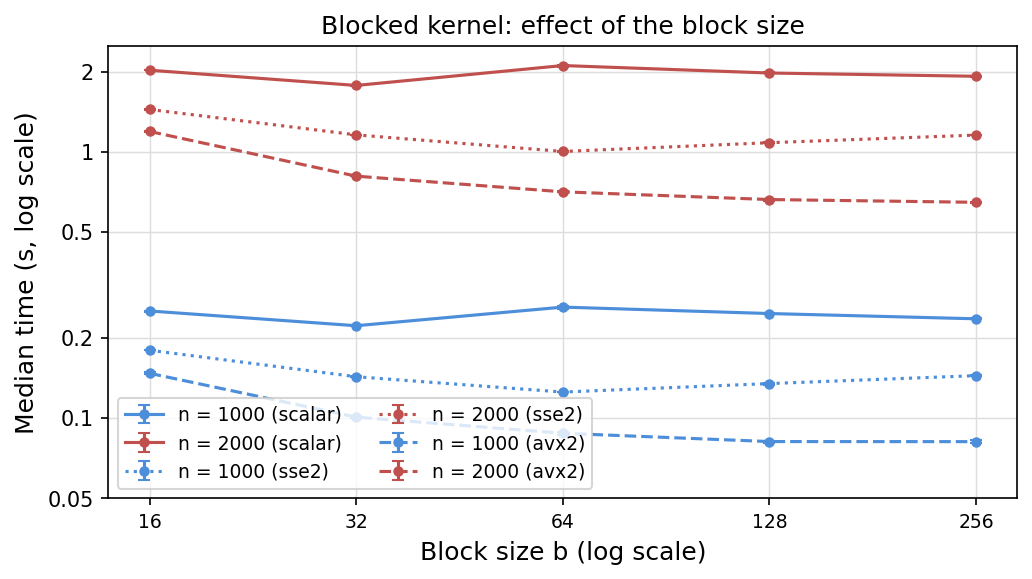
\includegraphics[width=0.72\textwidth]{../results/plot_block_size.png}
    \caption{Median time of the blocked kernel vs block size $b$ (log-log scale). Solid:
    scalar build; dashed: AVX2 build.}
    \label{fig:blocksize}
\end{figure}

\subsection{Part A: runtime of the dense methods}

Tables~\ref{tab:dense} and~\ref{tab:speedup} and Figures~\ref{fig:densetime}
and~\ref{fig:costperop} give the runtime of every dense configuration; every derived
number quoted below is computed by \texttt{analysis/report\_numbers.py}.

\begin{table}[htbp]
\centering
\footnotesize
\setlength{\tabcolsep}{2.5pt}
\begin{tabular}{rlllll}
\toprule
\textbf{n} & \textbf{ijk (s)} & \textbf{ikj (s)} & \textbf{blocked (s)} &
\textbf{transposed (s)} & \textbf{transpose (s)} \\
\midrule
\tableinput{../results/tables/dense_runtime.tex}
\bottomrule
\end{tabular}
\caption{Scalar build: median time per multiplication in seconds, with the IQR as a
percentage of the median in parentheses. \textit{transpose} is the transposition of $B$
alone, not included in \textit{transposed}. Every value comes from 15 measured runs in
3 processes, except \texttt{ijk} at $n = 3000$ and 4000 (5 runs in one process). For
$n \le 200$ each run is a batch of calls lasting at least 10~ms.}
\label{tab:dense}
\end{table}

\begin{table}[htbp]
\centering
\footnotesize
\setlength{\tabcolsep}{3.5pt}
\begin{tabular}{rrrrrrrrrrrrrr}
\toprule
& \multicolumn{7}{c}{\textbf{ns per multiply-add}} & \multicolumn{6}{c}{\textbf{Speedup
over scalar \texttt{ijk}}} \\
\cmidrule(lr){2-8} \cmidrule(lr){9-14}
& \multicolumn{4}{c}{scalar} & \multicolumn{3}{c}{AVX2} & \multicolumn{3}{c}{scalar} &
\multicolumn{3}{c}{AVX2} \\
\cmidrule(lr){2-5} \cmidrule(lr){6-8} \cmidrule(lr){9-11} \cmidrule(lr){12-14}
\textbf{n} & ijk & ikj & blk & tr & ikj & blk & tr & ikj & blk & tr & ikj & blk & tr \\
\midrule
\tableinput{../results/tables/dense_speedup.tex}
\bottomrule
\end{tabular}
\caption{Median time divided by $n^3$ (nanoseconds per multiply-add) and median time of
scalar \texttt{ijk} divided by the median time of each method at the same $n$ (blk:
blocked; tr: transposed, without the transposition).}
\label{tab:speedup}
\end{table}

\begin{figure}[htbp]
    \centering
    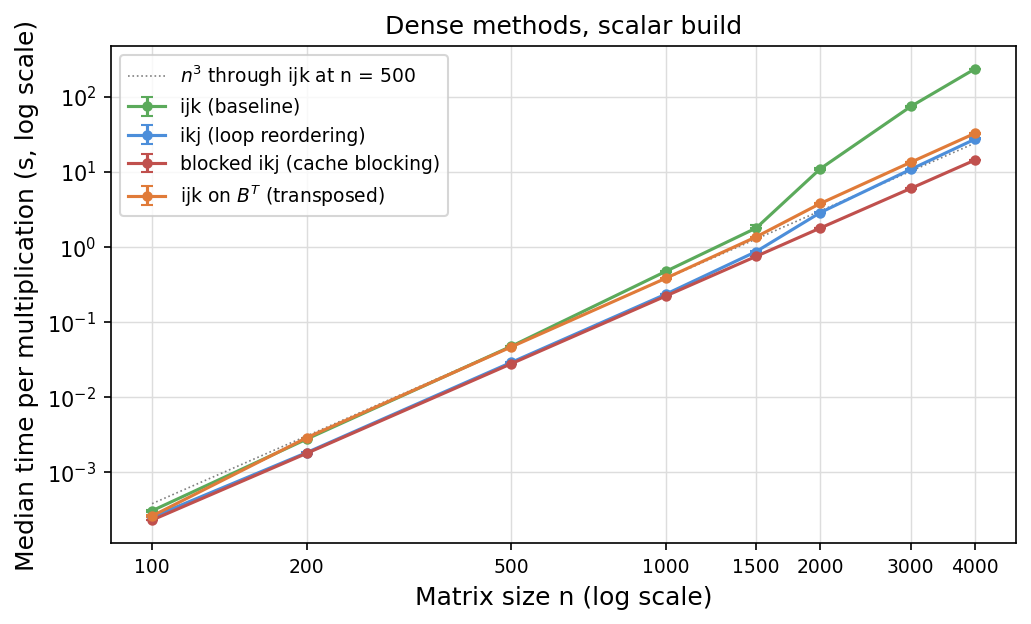
\includegraphics[width=0.8\textwidth]{../results/plot_dense_time.png}
    \caption{Median time per multiplication of the dense methods in the scalar build vs
    matrix size $n$ (log-log scale). The dotted line is the cubic model through
    \texttt{ijk} at $n = 500$. Error bars show the IQR (smaller than the markers).}
    \label{fig:densetime}
\end{figure}

\begin{figure}[htbp]
    \centering
    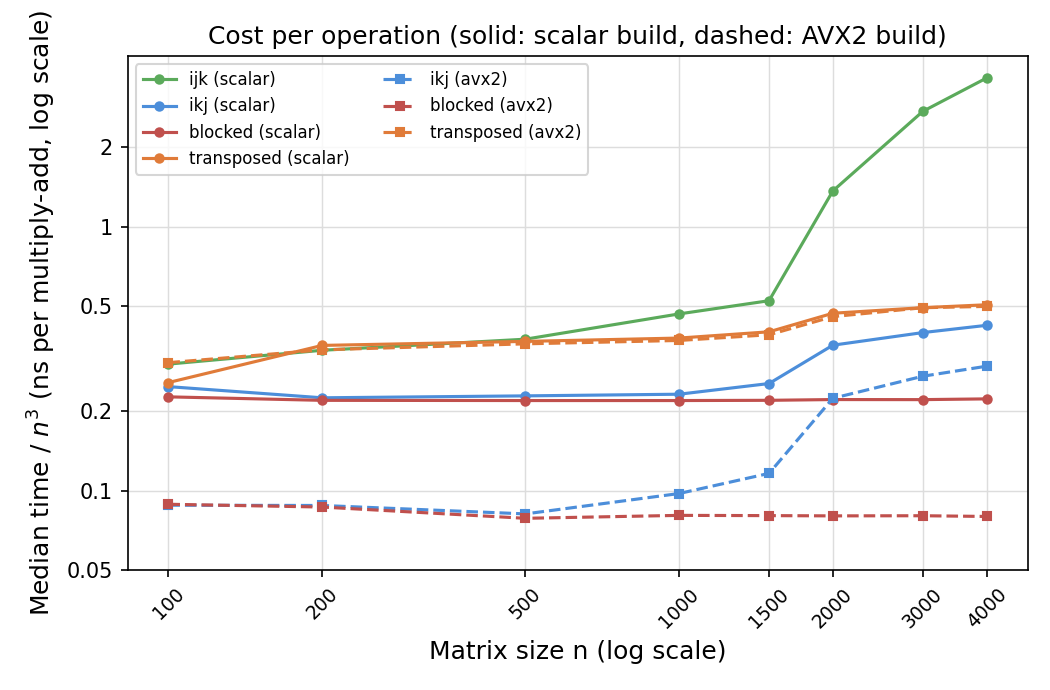
\includegraphics[width=0.8\textwidth]{../results/plot_cost_per_op.png}
    \caption{Median time divided by $n^3$ (nanoseconds per multiply-add), both builds. If
    the runtime were exactly proportional to $n^3$, each line would be horizontal.}
    \label{fig:costperop}
\end{figure}

\textit{Loop order and blocking.} \texttt{ikj} is faster than \texttt{ijk} at every size,
by a factor that grows from 1.6 at $n = 500$ and 2.0--2.1 at $n = 1000$--$1500$ to 3.8 at
$n = 2000$ and 8.6 at $n = 4000$. Its cost per multiply-add is 0.23~ns up to $n = 1000$ and
then rises to 0.25, 0.36 and 0.42~ns at $n = 1500$, 2000 and 4000; \texttt{ijk} rises from
0.52 to 1.36~ns between $n = 1500$ and 2000 and reaches 3.65~ns at $n = 4000$. The blocked
kernel keeps 0.219--0.222~ns from $n = 500$ to $4000$ (fitted exponent 3.01): it is 1.02--1.16
times faster than \texttt{ikj} up to $n = 1500$ and 1.61, 1.79 and 1.90 times faster at
$n = 2000$, 3000 and 4000, and 16.4 times faster than \texttt{ijk} at $n = 4000$.

\textit{Transposed operand.} The \texttt{transposed} kernel takes 0.96--1.02 times the
time of \texttt{ijk} at $n = 200$ and $500$ (0.36--0.37~ns per multiply-add in both) and
is faster from $n = 1000$ (1.23 times) to $n = 4000$ (7.2 times). It is slower than
\texttt{ikj} at every size, by 1.6 times for $200 \le n \le 1500$ and 1.2 times at
$n = 4000$. The transposition itself takes 0.15--0.5\% of the time of the
\texttt{transposed} kernel for $n \ge 200$, so adding it changes the speedup over
\texttt{ijk} by at most 0.01.

\textit{Vectorisation.} The AVX2 build makes the blocked kernel 2.54--2.79 times faster at
every size (0.080~ns per multiply-add from $n = 500$ to $4000$). For \texttt{ikj} the gain
falls with $n$: 2.2--2.8 times up to $n = 1500$, 1.59 at $n = 2000$ and 1.43 at
$n = 4000$, where the vectorised \texttt{ikj} needs 3.71 times the time of the vectorised
blocked kernel. The \texttt{transposed} kernel, which has no vector code, takes
0.96--1.00 times its scalar time from $n = 200$; at $n = 100$ the AVX2 build is 16\%
slower (0.305 against 0.257~ns). The fastest configuration, the vectorised blocked kernel,
is 3.4--6.5 times faster than \texttt{ijk} up to $n = 1500$ and 17.0, 34.0 and 45.8 times
faster at $n = 2000$, 3000 and 4000.

\textit{Variability.} The IQR is at most 3\% of the median in 78.5\% of the 214
configurations of the study. Among the configurations with a median above 1~ms, the
largest values are those of the transposition alone (up to 33.4\% at $n = 2000$, where a
call lasts 6~ms), \texttt{ijk} at $n = 1500$ (9.4\%) and in the density experiment at
$n = 2000$ (up to 13.5\%, with process medians up to 22\% apart), and the vectorised
\texttt{ikj} at $n = 1500$ (10.8\%). Every configuration ran in 3 processes except
\texttt{ijk} at $n = 3000$ and 4000 (one process, medians of 74 and 234~s).

\subsection{Part A: memory}

Table~\ref{tab:memdense} gives the peak working set of the dense methods. It is identical
for \texttt{ijk}, \texttt{ikj} and the blocked kernel, and for $n \ge 1000$ grows by 24.0
bytes per matrix element: the three float64 matrices, plus about 4~MiB of fixed program
memory. \texttt{transposed} grows by 32.0 bytes per element, because it also holds $B^T$.
None of the optimisations needs more memory than the baseline except the transposed
operand, which needs one more matrix.

\begin{table}[htbp]
\centering
\small
\begin{tabular}{rrrrrr}
\toprule
& \multicolumn{4}{c}{\textbf{Peak working set (MiB)}} & \\
\textbf{n} & \textbf{ijk} & \textbf{ikj} & \textbf{blocked} & \textbf{transposed} &
\textbf{$24n^2$ bytes (MiB)} \\
\midrule
\tableinput{../results/tables/memory_dense.tex}
\bottomrule
\end{tabular}
\caption{Peak working set of the dense methods in the scalar build (median over processes,
MiB $= 2^{20}$ bytes) and computed storage of three float64 matrices. The computed storage
of \texttt{transposed} is $32n^2$ bytes.}
\label{tab:memdense}
\end{table}

\subsection{Part B: density at fixed size}

Table~\ref{tab:density} and Figures~\ref{fig:densitytime}--\ref{fig:densitymemory} give the
results at $n = 2000$. The densities of the generated inputs are within 0.02 percentage
points of the requested ones.

\begin{table}[htbp]
\centering
\footnotesize
\setlength{\tabcolsep}{4pt}
\begin{tabular}{rrrlllllr}
\toprule
& \multicolumn{2}{c}{\textbf{Density (\%)}} & & & \multicolumn{2}{c}{\textbf{Dense
blocked (s)}} & \multicolumn{2}{c}{\textbf{Scalar blocked /}} \\
\cmidrule(lr){2-3} \cmidrule(lr){6-7} \cmidrule(lr){8-9}
\textbf{d (\%)} & \textbf{A} & \textbf{C} & \textbf{CSR (s)} & \textbf{Conv. (s)} &
\textbf{scalar} & \textbf{AVX2} & \textbf{CSR} & \textbf{CSR + conv.} \\
\midrule
\tableinput{../results/tables/density.tex}
\bottomrule
\end{tabular}
\caption{$n = 2000$. Requested density $d$, measured density of $A$ and of the product $C$,
median times of the CSR kernel, of the conversion of $A$ and $B$ to CSR and of the dense
blocked kernel, and ratio of the scalar blocked time to the CSR time without and with the
conversion. A ratio above 1 means that CSR is faster.}
\label{tab:density}
\end{table}

\begin{figure}[htbp]
    \centering
    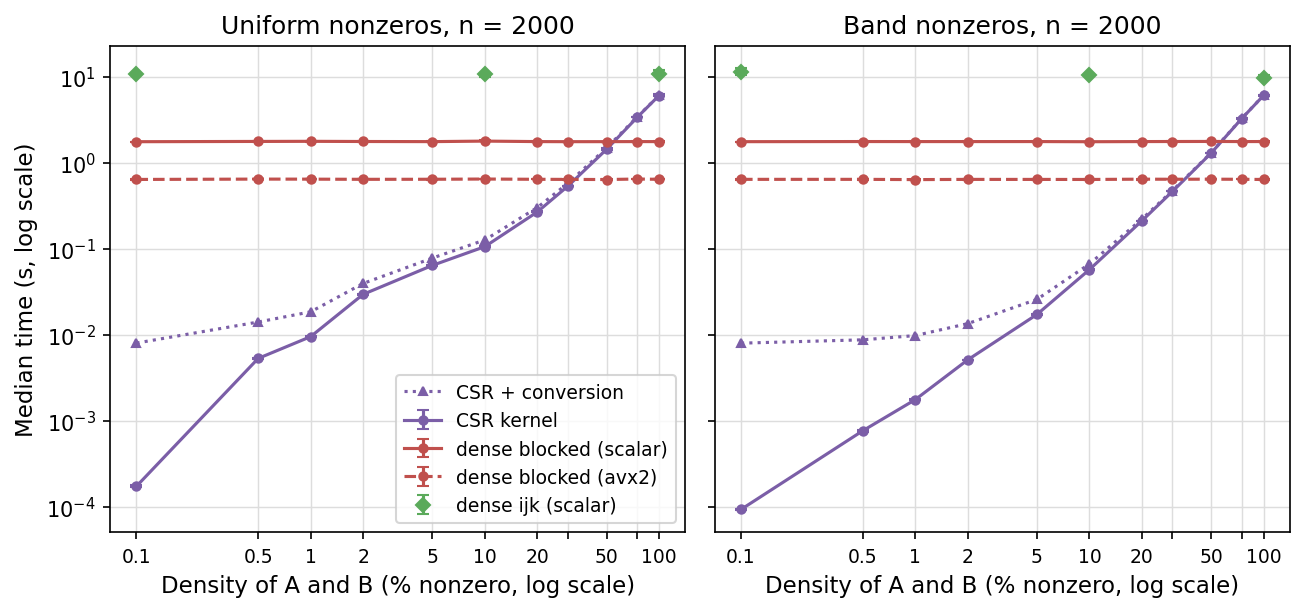
\includegraphics[width=\textwidth]{../results/plot_density_time.png}
    \caption{Median time vs density of $A$ and $B$ at $n = 2000$ (log-log scale). Left:
    uniform nonzeros; right: band nonzeros. The dense \texttt{ijk} was run at three
    densities only.}
    \label{fig:densitytime}
\end{figure}

\begin{figure}[htbp]
    \centering
    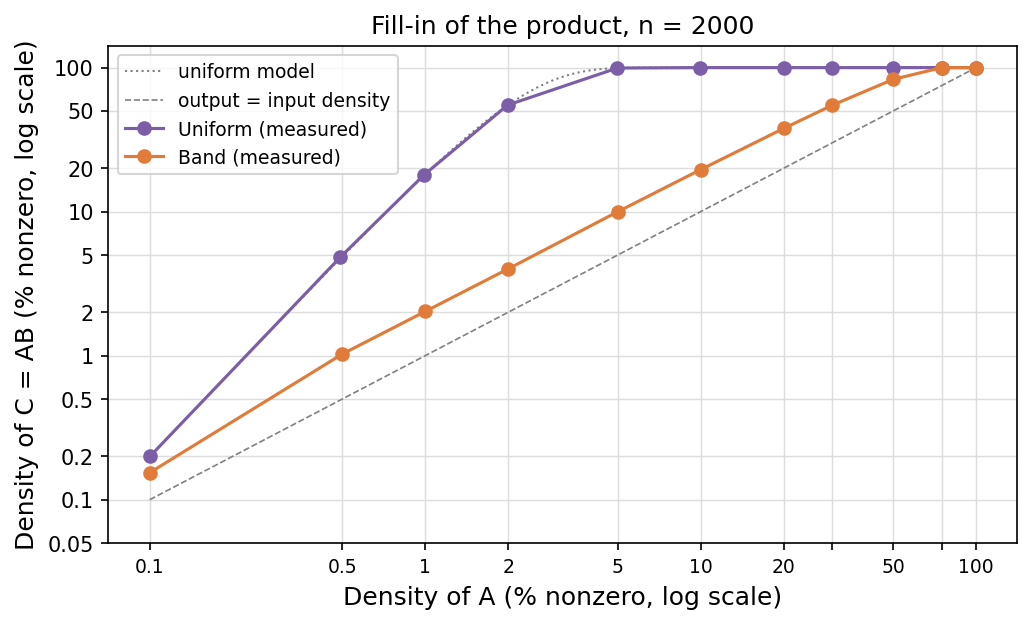
\includegraphics[width=0.8\textwidth]{../results/plot_output_density.png}
    \caption{Density of the product $C = AB$ vs density of the inputs at $n = 2000$
    (log-log scale). The dotted line is the uniform model $1 - (1 - d^2)^n$.}
    \label{fig:fillin}
\end{figure}

\begin{figure}[htbp]
    \centering
    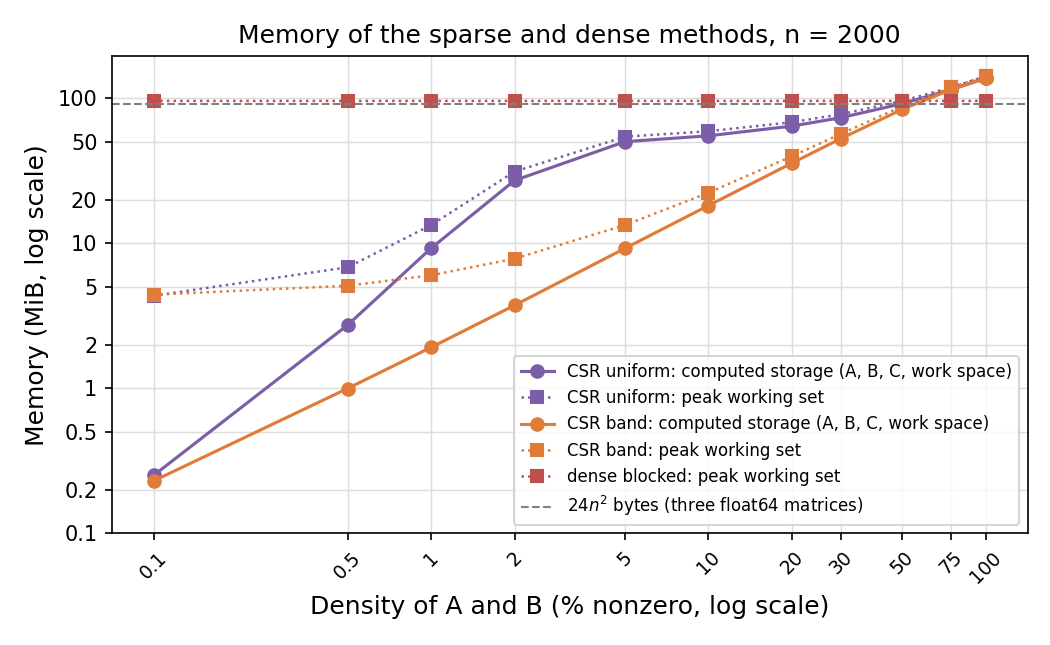
\includegraphics[width=0.8\textwidth]{../results/plot_density_memory.png}
    \caption{Memory vs density at $n = 2000$ (log-log scale): computed storage of the CSR
    matrices $A$, $B$, $C$ and work space, and peak working set of the CSR and dense
    blocked processes. The dashed line is $24n^2$ bytes.}
    \label{fig:densitymemory}
\end{figure}

\textit{Dense methods.} The dense kernels do not depend on the zeros: across the 22 inputs
the median of the blocked kernel varies by 1.6\% in each build (1.758--1.787~s scalar,
0.638--0.648~s AVX2), and \texttt{ijk} took 9.8--11.5~s, against 10.9~s on the dense
matrices.

\textit{Fill-in.} For uniform inputs the measured density of $C$ follows the model
$1 - (1 - d^2)^n$ (Figure~\ref{fig:fillin}): 18\% at $d = 1\%$, 55\% at $d = 2\%$ and
99.3\% at $d = 5\%$, so from $d = 5\%$ the product is practically dense. For band inputs
the density of $C$ is 1.5--2.1 times that of the inputs up to $d = 20\%$ (37.8\%), and the
product reaches 100\% only at $d = 75\%$.

\textit{Time.} The CSR kernel is faster than the scalar blocked kernel up to $d = 50\%$
in both distributions: by 10\,100 (uniform) and 18\,900 (band) times at $d = 0.1\%$,
187 and 1000 times at $d = 1\%$, 16.9 and 30.7 times at $d = 10\%$, and 1.23 and 1.37 times
at $d = 50\%$. At $d = 75\%$ and $100\%$ it needs 1.9 and 3.4 times the dense time. At
every density from 0.1\% to 50\% the advantage is larger for band inputs. Interpolating
the ratio in logarithmic scale, the time crossover is at 55.1\% (uniform) and 57.3\%
(band) against the scalar blocked kernel, and at 32.9\% and 35.3\% against the vectorised
one. Divided by $n^3 d^2$, the CSR time is 0.72--0.76~ns (uniform) and 0.65--0.76~ns (band)
for $d \ge 20\%$, and grows at low density, up to 21.7 and 11.6~ns at $d = 0.1\%$.

\textit{Conversion.} Converting $A$ and $B$ to CSR takes 7.8--53~ms. It costs 45 (uniform)
and 85 (band) times the CSR kernel at $d = 0.1\%$, about as much as the kernel at 0.5--1\% (uniform) and 2--5\% (band),
and less than 20\% of it from $d = 10\%$. Including it moves the crossovers by at most
1.2 percentage points (54.3\% and 57.1\% against the scalar kernel) and leaves CSR 219
and 220 times faster than the scalar dense kernel at $d = 0.1\%$. For uniform inputs the
conversion time is highest at $d = 50\%$ (52.9~ms) and falls to 17.5~ms at $d = 100\%$;
for band inputs it grows steadily with $d$.

\textit{Memory.} The computed storage of the CSR matrices is smaller than the $24n^2$
bytes of the three dense matrices up to 49.9\% density (uniform) and 56.1\% (band), and
1.5 times larger at 100\%. At $d = 5\%$, with an almost full product, the uniform CSR
matrices still need 0.55 times the dense storage. The peak working set follows the same
pattern: 4.3~MiB at $d = 0.1\%$ and 141.5~MiB at $d = 100\%$ for CSR, against 95.6~MiB for
the dense blocked kernel at every density.

\subsection{Part B: matrix size at fixed density}

Table~\ref{tab:size} and Figure~\ref{fig:size} give the CSR results from $n = 1000$ to
$32\,000$. The fitted exponents of the CSR time over this range are 3.33 (uniform 0.1\%),
2.74 (uniform 1\%), 2.46 (band 0.1\%) and 2.52 (band 1\%). At a fixed density the
uniform products fill in as $n$ grows (from 9.4\% to 95.9\% at $d = 1\%$), while the band
products keep a constant density (0.2\% and 2.0\%). On the inputs where both ran
($n \le 4000$), CSR is 158--24\,300 times faster than the scalar blocked kernel.

\begin{table}[htbp]
\centering
\small
\begin{tabular}{llrlrrrl}
\toprule
\textbf{Distr.} & \textbf{d (\%)} & \textbf{n} & \textbf{CSR (s)} & \textbf{C (\%)} &
\textbf{Storage} & \textbf{Peak} & \textbf{Blocked (s)} \\
\midrule
\tableinput{../results/tables/size.tex}
\bottomrule
\end{tabular}
\caption{CSR multiplication at fixed density: median time (IQR in parentheses), density of
the product, computed storage and peak working set (MiB), and the scalar dense blocked
kernel on the same inputs (run up to $n = 4000$).}
\label{tab:size}
\end{table}

\begin{figure}[htbp]
    \centering
    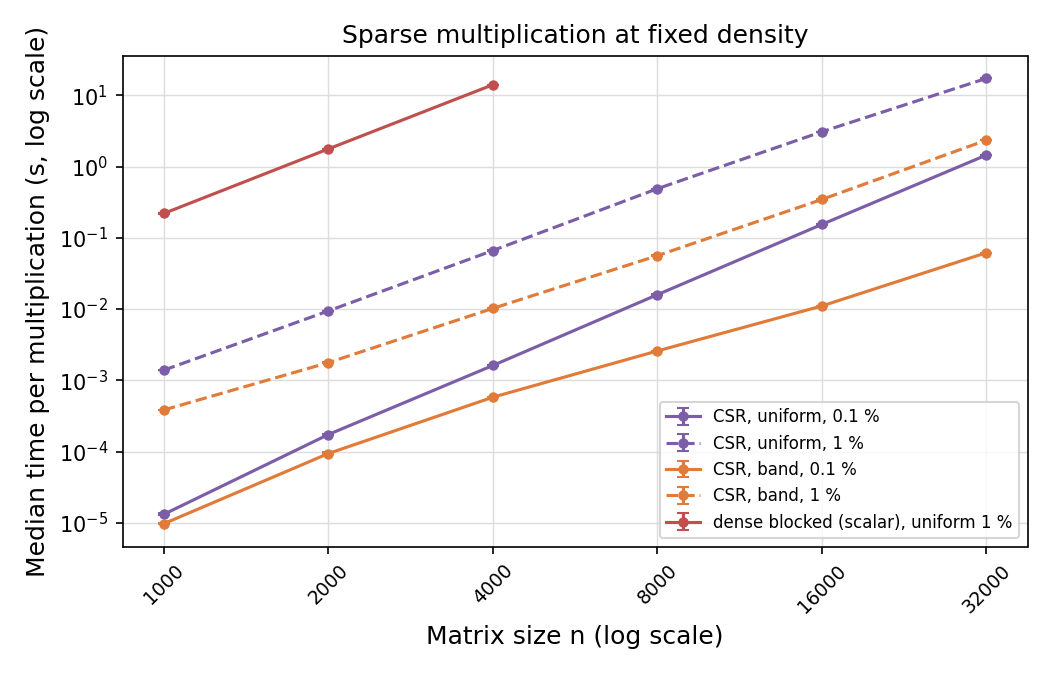
\includegraphics[width=0.8\textwidth]{../results/plot_size_time.png}
    \caption{Median time of the CSR multiplication at fixed density vs matrix size $n$
    (log-log scale), and the dense blocked kernel (scalar) up to $n = 4000$.}
    \label{fig:size}
\end{figure}

\subsection{Largest feasible size}

No process exceeded the time or memory budget, so every declared size finished
(\texttt{results/run\_status.csv}). Table~\ref{tab:limits} summarises the limits.

\begin{table}[htbp]
\centering
\small
\begin{tabular}{llll}
\toprule
\textbf{Method} & \textbf{Largest feasible $n$} & \textbf{Longest median} &
\textbf{Largest peak} \\
\midrule
\texttt{ijk} (scalar) & 4000 & 234~s & 370~MiB \\
\texttt{ikj} / blocked (scalar) & 4000 & 27.0~s / 14.2~s & 370~MiB \\
blocked (AVX2) & 4000 & 5.1~s & 370~MiB \\
\texttt{transposed} (scalar) & 4000 & 32.4~s & 492~MiB \\
CSR, uniform 1\% & 32\,000 & 17.3~s & 11\,481~MiB \\
CSR, band 1\% & 32\,000 & 2.35~s & 473~MiB \\
\bottomrule
\end{tabular}
\caption{Limits under the budget of 15~minutes per run and 16~GiB of matrix storage. The
largest sizes attempted were $n = 4000$ for the dense methods and $32\,000$ for CSR; none
exceeded the budget.}
\label{tab:limits}
\end{table}

\FloatBarrier
\section{Discussion}

\subsection{Evaluation of the hypotheses}

In answer to question~(A): reading memory with unit stride and reusing tiles from the
cache remove most of the slowdown of \texttt{ijk} at large $n$ without extra memory, and
vectorisation multiplies the gain of the kernels that gcc can vectorise. In answer to
question~(B): at $n = 2000$, CSR is faster than the dense kernels up to a density of
about one half against the scalar kernel and one third against the vectorised one, and
needs less storage up to about one half, for both distributions. Table~\ref{tab:verdicts}
gives the verdict for each prediction.

\begin{table}[H]
\centering
\small
\begin{tabular}{p{2.2cm}p{8.0cm}>{\raggedright\arraybackslash}p{3.0cm}}
\toprule
\textbf{Prediction} & \textbf{Observed} & \textbf{Verdict} \\
\midrule
P1 Loop order & \texttt{ikj} faster at every $n \ge 500$ (1.6--8.6 times), but its cost
per multiply-add still rises from 0.25 to 0.36~ns between $n = 1500$ and 2000 & Partly
confirmed (smaller jump, not none) \\
\addlinespace
P2 Blocking & 1.61--1.90 times faster than \texttt{ikj} for $n \ge 2000$; constant
0.22~ns per multiply-add & Confirmed \\
\addlinespace
P3 Transposed & Slower than \texttt{ikj} at every size; faster than \texttt{ijk} only from
$n = 1000$, equal within 4\% for $200 \le n \le 500$ & Partly confirmed (not faster
below $n = 1000$) \\
\addlinespace
P4 Vectorisation & Blocked 2.5--2.8 times, \texttt{ikj} 1.4--2.8 times, the non-vectorised
\texttt{transposed} within 4\% from $n = 200$ & Confirmed \\
\addlinespace
P5 Sparse time & CSR faster than scalar blocked up to 50\% (crossovers 55\% and 57\%);
larger advantage for band inputs at every density up to 50\% & Confirmed \\
\addlinespace
P6 Sparse memory & CSR storage smaller than dense up to 50\% (uniform) and 56\% (band),
including uniform inputs with $5\% \le d \le 50\%$ & Refuted (threshold wrong) \\
\bottomrule
\end{tabular}
\caption{Verdict for each prediction of Table~\ref{tab:predictions}.}
\label{tab:verdicts}
\end{table}

\subsection{Effect of the dense optimisations}

\textit{Memory access.} The four dense kernels perform the same $n^3$ multiply-adds in the
same order for each element, so their differences come from the order in which memory is
read. For $n \le 1500$, $B$ (at most 18~MB) fits in the 30~MB L3, and
\texttt{ikj} is 1.6--2.1 times faster than \texttt{ijk}. Beyond that size the column walk
of \texttt{ijk} becomes 2.6 times more expensive per operation, while \texttt{ikj} rises
by 40\%. \texttt{ikj} reads $B$ row by row, so every page and cache line it touches is used
completely; its smaller jump is therefore consistent with the L3-capacity explanation of
Assignment~1 (the whole of $B$, 32~MB at $n = 2000$, is read again from memory for every
row of $C$), and suggests that the much larger jump of \texttt{ijk} comes from its stride
in addition. Neither the TLB nor the cache misses were measured, so the share of each
effect remains a hypothesis. At $n = 2000$, \texttt{ikj} reads one 8-byte element of $B$
per multiply-add, which at 0.36~ns (scalar) and 0.22~ns (AVX2) is equivalent to about 22
and 36~GB/s, plausible main-memory rates; no bandwidth benchmark was run to confirm that
these are the limit.

The blocked kernel removes the dependence on $n$: its cost per multiply-add is the same
from $n = 500$ to 4000, as expected if each tile of $B$ is reused from the cache by the
$b$ rows of a tile of $A$ instead of being read again from memory~\cite{lam1991}. The
best block sizes are consistent with the cache sizes, but this was not verified directly:
with $b = 32$ the three tiles occupy $3 \times 8b^2 = 24$~KB, within the 48~KB L1, and with
$b = 256$ they occupy 1.5~MB, within the 2~MB L2. In the scalar build all the block sizes
are within 19\%, so the exact choice matters little; in the AVX2 build, small tiles are
1.8 times slower, consistent with the inner loop over $b$ elements being too short for the
vector loop (4 doubles per instruction, unrolled 4 times) and the run-time aliasing check
that precedes it.

\textit{The transposed operand.} Transposing $B$ gives \texttt{ijk} unit stride but keeps
its dot product, one serial chain of $n$ additions per element. Up to $n = 500$, where
\texttt{ijk} still finds $B$ in the cache, both kernels cost 0.36--0.37~ns per
multiply-add, while \texttt{ikj}, whose consecutive additions go to different elements,
costs 0.23~ns. This is consistent with the dot-product kernels being limited by the
latency of the chain of additions rather than by memory~\cite{hennessy2019}; it was not
measured with hardware counters. The transposition itself costs almost nothing (at most
0.5\% of the kernel time), so the transposed operand is a valid fix for the memory
problem of \texttt{ijk} but not as good as reordering the loops.

\textit{Vectorisation.} Separating the build from the method shows that the order of the
loops is what allows vectorisation: the inner loop of \texttt{ikj} updates independent
elements of $C$ and is vectorised, whereas the dot product cannot be vectorised without
changing the rounding, and \texttt{transposed} gains nothing. The gain never reaches the
4 doubles of an AVX2 register (at most 2.8), and in \texttt{ikj} it falls to 1.4 at large
$n$: once the arithmetic is 2.5--2.8 times faster, the kernel that reads $B$ from memory
for every row spends a larger share of its time waiting for memory, which the blocked
kernel avoids. The two optimisations therefore combine: blocking alone gives 16.4 times
over \texttt{ijk} at $n = 4000$, vectorisation alone (\texttt{ikj}) 12.4 times with the
loop reordering it needs, and both together 45.8 times. The 16\% slowdown of the
non-vectorised \texttt{transposed} at $n = 100$ is not explained by the measurements; the
code is the same in both builds, so a difference in code alignment is one possible cause.

\subsection{Effect of sparse storage}

The CSR kernel avoids all the products with a zero factor, about $n^3 (1 - d^2)$ of the
$n^3$ multiply-adds, but pays more for each product it performs. For $d \ge 20\%$ its
time divided by $n^3 d^2$ is 0.65--0.76~ns, 3.0--3.5 times the 0.22~ns of the scalar blocked
kernel and 8--9.5 times the 0.080~ns of the vectorised one: each product reads a column
index, updates the accumulator at a scattered position and checks a marker. If both costs
were constant, the crossover would be where $d^2$ equals their ratio, at
$\sqrt{0.22 / 0.72} \approx 55\%$ against the scalar kernel and
$\sqrt{0.080 / 0.72} \approx 33\%$ against the vectorised one, close to the measured 55\%
and 33\% (uniform). The crossover thus depends on how optimised the dense kernel is: the
vectorisation of the dense kernel moves it from one half to one third.

At low density the cost per product grows (up to 21.7~ns at $d = 0.1\%$), because the
number of products falls as $d^2$ while some costs do not: the $n$ rows of $C$, the
initialisation of the markers and the sorting of each row of $C$. These costs grow with
the nonzeros of $C$, which is why the distribution matters: at $d = 1\%$ both distributions
perform about the same number of products, but the uniform product has 18\% nonzeros and
the band product 2\%, and the band kernel is 5.4 times faster. The band rows of $B$ that a
row of $A$ selects are also adjacent in memory, which may help; this was not separated
from the effect of the fill-in.

The conversion of the inputs is negligible at medium and high densities but dominates at
very low density (7.8~ms against 0.17~ms for the kernel at $d = 0.1\%$, uniform): its
time is bounded below by reading the $2 \times 8n^2$ bytes of the two dense matrices
twice. Even so, CSR with conversion remains about 220 times faster than the scalar
dense kernel at $d = 0.1\%$. The peak of the uniform conversion time at $d = 50\%$ is
consistent with the branch \texttt{if (v != 0)} of the copy pass being unpredictable when
half of the random entries are zero, which is not the case for band inputs, whose
nonzeros form almost contiguous runs (each band position is kept with probability
above 0.95 from $d = 1\%$); branch mispredictions were not measured.

\textit{Memory.} Prediction P6 compared the 12 bytes of a CSR nonzero with the 8 bytes of a
dense entry for the product only. The comparison that matters is with all three dense
matrices: even when $C$ is full and its CSR form needs $12n^2$ bytes, 1.5 times its dense
form, the sparse $A$ and $B$ save more than that up to about $d = 50\%$. Above it, CSR
needs up to 1.5 times the dense storage, and its peak working set at $d = 100\%$ is
141.5~MiB against 95.6~MiB.

\textit{Scaling.} At a fixed density the number of products grows as $n^3 d^2$, but the
measured exponents are not 3. For band inputs (2.5) the fixed per-row costs dominate at
small $n$ and are amortised as $n$ grows: the time per product of band 1\% falls from 3.8~ns
at $n = 1000$ to 0.71~ns at $32\,000$. For uniform inputs at 0.1\% the exponent is above 3:
the rows of $C$ have about $d^2 n^2$ nonzeros (about 1000 at $n = 32\,000$), which are
sorted with \texttt{qsort}, so the cost per product grows with $\log n$; this is consistent
with, but was not confirmed by, a profile of the kernel. The scaling experiment also shows
the main limit of sparse storage: uniform inputs with 1\% density give a product with 96\%
nonzeros at $n = 32\,000$, and the CSR storage (11.2~GiB, mostly $C$) is larger than the
7.6~GiB of a dense $C$. For comparison, three dense matrices would need $24n^2$ bytes,
22.9~GiB, above the 16~GiB budget, and the cubic extrapolation of the blocked kernel
gives about 2~hours per run; neither was run. Band inputs, whose product stays sparse,
needed 473~MiB at the same size.

\subsection{Limitations}

\begin{itemize}
    \item One Windows computer, one compiler and one set of flags; other cache sizes would
    move the jumps of the dense kernels, the best block size and the crossovers. The power
    plan was the default \textit{Balanced}, not a fixed frequency.
    \item The block size was chosen among five powers of two at one size; rectangular
    tiles, register blocking and the cache-oblivious recursion were not tested, so the
    blocked kernel is not the fastest possible dense kernel. The densities tested are 11
    values, and the crossovers between them are interpolated.
    \item The cache, TLB, latency and branch-prediction explanations are inferred from
    timings only; no hardware counters or profiles were used.
    \item Part~B was measured at $n = 2000$ only, and with two nonzero distributions; the
    crossovers depend on $n$ through the fill-in, and other patterns (block, power-law
    rows) may behave differently.
    \item The CSR implementation was not compared with an optimised library, and its
    sorting rule ($n/16$) was not tuned.
    \item \texttt{ijk} at $n = 3000$ and 4000 ran in one process (5 runs); \texttt{ijk} at
    $n = 2000$ showed process medians up to 22\% apart, so its single-process values may
    underestimate the uncertainty.
    \item No configuration reached the budget, so the actual largest feasible sizes were
    not determined.
\end{itemize}

\section{Conclusions}

For the programs and the conditions described in Section~3:
\begin{itemize}
    \item Changing only the order of memory accesses makes the dense multiplication much
    faster at the same number of operations and with the same memory: \texttt{ikj} is
    1.6--8.6 times faster than \texttt{ijk} for $500 \le n \le 4000$ and the blocked
    kernel 1.7--16.4 times. The blocked kernel keeps a constant cost of 0.22~ns per
    multiply-add up to $n = 4000$, and the jump of Assignment~1 does not appear in it.
    \item Transposing $B$ also removes most of the slowdown of \texttt{ijk} at large $n$,
    at a negligible cost and one more matrix of memory, but remains 1.2--1.6 times slower
    than \texttt{ikj}.
    \item Compiler vectorisation multiplies the effect of the optimisations it can be
    applied to: 2.5--2.8 times for the blocked kernel, up to 45.8 times faster than
    \texttt{ijk} at $n = 4000$, and nothing for the dot-product kernel.
    \item At $n = 2000$, CSR is faster than the dense blocked kernel up to a density of
    about 55--57\% (scalar) and 33--35\% (vectorised), by four orders of magnitude at
    0.1\%, and needs less storage up to 50--56\%. Its advantage at a given density is
    larger when the product stays sparse (band) than when it fills in (uniform).
    \item The conversion to CSR is negligible except at very low densities, where it costs
    up to 85 times the sparse kernel without changing the conclusion.
\end{itemize}
These results describe specific implementations on one machine. The effect of the
optimisations is to make each operation cheaper; the effect of sparse storage is to avoid
operations at a higher cost per operation, so its advantage depends both on the density
and on how fast the dense alternative is. Two questions remain open: which share of the
slowdown of the dense kernels comes from the cache and which from address translation,
which hardware counters could answer, and how the crossovers move with $n$ and with the
use of several threads.

\section*{Reproducibility materials}

The repository linked on the first page contains the source code, the build and run
commands (\texttt{README.md}) and, in \texttt{results}, the raw measurements of every
run, the status and peak memory of every process, the patterns of the sparse inputs, the
block size chosen, the compiler vectorisation report, the environment record and the
correctness results. The study is reproduced on Windows with \texttt{run\_experiment.py}
(build and benchmarks, 3.3~hours of benchmark processes on the machine described above),
the validation script \texttt{analysis/check\_correctness.py},
\texttt{analysis/plot\_results.py} (figures and tables) and
\texttt{analysis/report\_numbers.py} (every other number in the text).

\section*{Use of generative AI}

Claude Opus 5.5 (Anthropic), used through Claude Code, was used during this assignment to
help write and debug the benchmark, run and analysis code, and to draft and revise the
text of the report from the measured results. All the measurements come from running the
code on the machine described above. The author defined the study, reviewed the code and
the AI-generated text, checked the numbers against the raw data and the references, and
is responsible for the conclusions.

\clearpage
{\small
\begin{thebibliography}{8}

\bibitem{cormen2009}
T.~H. Cormen, C.~E. Leiserson, R.~L. Rivest, and C.~Stein, \textit{Introduction to
Algorithms}, 3rd~ed. Cambridge, MA, USA: MIT Press, 2009.

\bibitem{hennessy2019}
J.~L. Hennessy and D.~A. Patterson, \textit{Computer Architecture: A Quantitative
Approach}, 6th~ed. Cambridge, MA, USA: Morgan Kaufmann, 2019.

\bibitem{goldberg1991}
D.~Goldberg, ``What every computer scientist should know about floating-point
arithmetic,'' \textit{ACM Comput. Surv.}, vol.~23, no.~1, pp.~5--48, Mar. 1991,
doi: 10.1145/103162.103163.

\bibitem{lam1991}
M.~D. Lam, E.~E. Rothberg, and M.~E. Wolf, ``The cache performance and optimizations of
blocked algorithms,'' in \textit{Proc. 4th Int. Conf. Architectural Support for
Programming Languages and Operating Systems (ASPLOS IV)}, 1991, pp.~63--74,
doi: 10.1145/106972.106981.

\bibitem{gustavson1978}
F.~G. Gustavson, ``Two fast algorithms for sparse matrices: multiplication and permuted
transposition,'' \textit{ACM Trans. Math. Softw.}, vol.~4, no.~3, pp.~250--269, 1978,
doi: 10.1145/355791.355796.

\bibitem{saad2003}
Y.~Saad, \textit{Iterative Methods for Sparse Linear Systems}, 2nd~ed. Philadelphia, PA,
USA: SIAM, 2003.

\bibitem{gccopt}
Free Software Foundation, ``Options that control optimization,'' in \textit{Using the GNU
Compiler Collection (GCC)}. [Online]. Available:
\url{https://gcc.gnu.org/onlinedocs/gcc/Optimize-Options.html}.

\bibitem{gccx86}
Free Software Foundation, ``x86 options,'' in \textit{Using the GNU Compiler Collection
(GCC)}. [Online]. Available: \url{https://gcc.gnu.org/onlinedocs/gcc/x86-Options.html}.

\end{thebibliography}
}


\end{document}
